\chapter{Design and Methodology}

\section{Introduction}

In this section the design and methodology choices involved in this project will be presented. This project consists of five main stages (Figure ~\ref{fig:pipeline}), each of which will be discussed in this chapter. These five stages are:
\begin{itemize}
    \item Data Collection and Filtering: Collecting the data and filtering it so it only contains tweet about hotels posted from Dublin.
    \item Dataset Annotation: Annotating the filtered dataset.
    \item Classification: Training and evaluating multiple supervised machine learning classifiers.
    \item Sentiment Analysis: Analysing the sentiment of the tweets classified as reviews.
    \item Application to Recommender System: Using the sentiment scores produced to re rank the results of the CoRE recommender system.
\end{itemize}

\begin{figure}[h!]
\centering
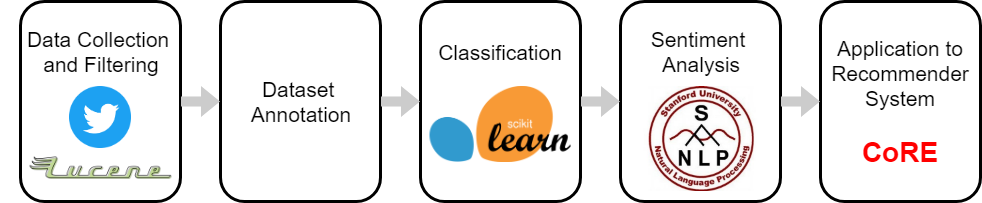
\includegraphics[width=1\textwidth]{design_and_methodology/pipeline.png}
\caption{\label{fig:pipeline} Overview of Project.}
\end{figure}

\section{Data Collection}
The data was collected using the Twitter Streaming API between October 2017 and September 2018. Twitter has a Search API and a Streaming API. The Search API allows you to find historical tweets and the Streaming API allows you to stream real-time tweets.

The data for this project was collected using the Streaming API. A filter was specified so that only tweets posted from within a bounding box of Dublin were returned. A total of 2.5 million tweets were collected.

After inspecting the collection of tweets it was found that although a bounding box had been specified not all tweets were posted from Dublin. A significant amount of tweets had slipped through Twitter's location filter. This meant the first step was to filter the dataset.

\section{Data Filtering}

\subsection*{Geo-tagged Tweets}

All of the tweets in the dataset were Geo-tagged. This meant they all had location data, a specified location from which the tweet was posted. There are two main types of Geo-tagged tweets:
\begin{itemize}
    \item Tweets with a specific latitude/longitude or 'Point' coordinate. These tweets come from GPS enabled devices (Listing ~\ref{lst:pointjson}).
    \item Tweets with a bounding box or Twitter 'Place'. A bounding box is a four-sided geographic area, defined by four points of the form [longitude, latitude]. This defines the general area the tweet was posted from (Listing ~\ref{lst:placejson}).
\end{itemize}

\begin{lstlisting}[caption={Geo-tagged Tweet with Point Coordinate},
captionpos=b,label=lst:pointjson,language=json,firstnumber=1]
"geo": {
    "type": "Point",
    "coordinates": 
        53.28581863,
        -6.11439315
    ]
}
\end{lstlisting}

\begin{lstlisting}[caption={Geo-tagged Tweet with Twitter Place},captionpos=b,label=lst:placejson,language=json,firstnumber=1]
"place": {
  "full_name": "Dun Laoghaire-Rathdown, Ireland",
  "url": "https://api.twitter.com/1.1/geo/id/723427e351a01e72.json",
  "country": "Ireland",
  "place_type": "city",
  "bounding_box": {
    "type": "Polygon",
    "coordinates": [
      [
        [
          -6.282038,
          53.199283
        ],
        [
          -6.282038,
          53.315283
        ],
        [
          -6.066759,
          53.315283
        ],
        [
          -6.066759,
          53.199283
        ]
      ]
    ]
  },
  "country_code": "IE",
  "attributes": {},
  "id": "723427e351a01e72",
  "name": "Dun Laoghaire-Rathdown"
}
\end{lstlisting}

\subsection*{Filtering Out Non-Dublin Tweets}

The first attempt to filter out any non Dublin tweets involved using the 'Point' coordinate of the tweets. The point coordinate of each tweet was compared to the bounding box of Dublin. If it lay inside the box it was kept, otherwise it was filtered out. However, only 7.23\% of the tweets in our collection had a specific 'Point' coordinate. Filtering based on this excluded the majority of the dataset. To address this we instead filtered tweets based on either their 'Point' coordinate or their Twitter 'Place'.

All of the tweets in the collection have a Twitter 'Place' defining the general area that the tweet was posted from. A combination of the Twitter 'Place' and the 'Point' coordinates was used to filter out any non Dublin tweets that had ended up in the dataset. 

\begin{table}[h!]
\caption{Coordinates for Dublin's Bounding Box}
\label{tab:dublinbb}
\begin{tabular}{|l|l|}
\hline
North Latitude  & 53.425210 \\ \hline
South Latitude  & 53.223430 \\ \hline
East Longitude & -6.043924 \\ \hline
West Longitude & -6.447485 \\ \hline
\end{tabular}
\end{table}

A bounding box for the Dublin area was defined (Table ~\ref{tab:dublinbb}). Then tweets with a 'Point' coordinate and tweets with only a Twitter 'Place' were treated differently:
\begin{itemize}
    \item \textbf{Point Coordinates}\newline
    Each tweet with a point coordinate was checked to see if it fell within the defined bounding box for Dublin. If it lay inside the box it was kept, otherwise it was filtered out.
    \item \textbf{Twitter Place}\newline
    Each tweet with a Twitter 'Place' has a bounding box specifying the 'Place'. The centroid of this bounding box was calculated for each tweet. Then the centroid was checked to see if it fell within the defined bounding box for Dublin. If it lay inside the box it was kept, otherwise it was filtered out.
\end{itemize}

The filtered dataset consisted of 1.6 million tweets posted from Dublin between October 2017 and September 2018.

\subsection*{Filter Out Tweets About Hotels}

Now that the dataset had been filtered so it only contained tweets posted from Dublin, the next step was to extract the tweets that mentioned hotels.

A list of the hotels in Dublin was compiled. This included the hotel's name and the hotel's Twitter handle (@hotelname). This list consisted of 0000 hotels and Twitter handles.

The tweets were stored in a Lucene index. A fuzzy search query was used to match the tweets against each of the hotel names and hotel Twitter handles. The fuzzy search query uses a similarity measure that is based on the Damerau-Levenshtein algorithm. The maximum edits option was set to two. This means that strings with a maximum difference of two characters would match. This accounted for misspellings and broadened our search slightly. Higher number of maximum edits were experimented with but we found that too many irrelevant tweets were returned.

This further filtered dataset consisted of 3000 tweets about hotels posted from Dublin between October 2017 and September 2018.

\section{Dataset Annotation}

One major goal of this research was to categorise tweets as review-like tweets, tweets that contain come content and irrelevant tweets. In order to train a classifier to do this a set of tweets had to first be manually annotated. The set of 3000 tweets about hotels in Dublin was annotated. This involved building an annotation webpage where users could view tweets and assign them a label.

\subsection*{Annotation Webpage}

A simple webpage was created in order to annotate the tweets (Figure ~\ref{fig:webpage}). The webpage can be found at \url{http://reviewtweets.epizy.com/}. The text of each tweet was displayed alongside three buttons; review, some content and irrelevant. The annotator could click on the option they thought best described the tweet shown. Once they chose a label, the next tweet would be displayed. 

\begin{figure}[h!]
\centering
\fbox{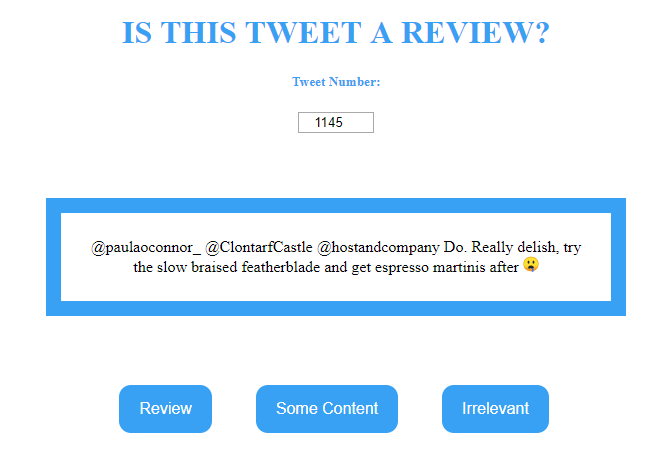
\includegraphics[width=1\textwidth]{design_and_methodology/webpage.PNG}}
\caption{\label{fig:webpage} Webpage for gathering Tweet Annotations.}
\end{figure}

Each time the webpage is loaded a random tweet from the dataset is displayed. The annotator can annotate the tweets incrementally from that random tweet on. This means each annotator will label a different section of the tweets, ensuring all tweets in the collection get annotated evenly.

The following instructions, describing what a review, some content and irrelevant tweet should look like accompanied the webpage:
\begin{itemize}
    \item \textbf{Review} \newline
    The tweet could be considered as a review (of any aspects related to a hotel such as the venue, food, view, swimming pool etc.) for any hotel. Examples would include: \emph{"Amazing view of the Aviva Stadium from my hotel balcony at hotel X"} (positive review), "Room service was awful at hotel Y" (negative review), \emph{"Thank you hotel X for a lovely stay"} (positive review) or \emph{"Had an awful night at hotel Y"} (negative review).
    \item \textbf{Some Content} \newline
    The tweet doesn't look like a review, but it does provide some information related to a hotel, such as the hotel hosts events, information on the menu, information related to accommodation etc. Examples would include: \emph{"Hotel Z serves Tuna salad on Wednesday”} or \emph{“A packed room for the 2018 fashion conference at Hotel X”}.
    \item \textbf{Irrelevant} \newline
    This tweet is completely irrelevant. While perhaps mentioning the name of a hotel, the tweet doesn't give any additional information about that hotel or offer any opinions related to the hotel.
\end{itemize}

In this research we decided to focus solely on the text of the tweets. For this reason all images, videos and URLs were removed from the tweets.

\begin{table}[h!]
\setlength\extrarowheight{5pt}
\begin{tabular}{|l|l|l|l|l|l|}
\hline
    \multicolumn{1}{|l|}{\textbf{Row No.}} & 
    \multicolumn{1}{l|}{\textbf{Tweet ID}} & 
    \multicolumn{1}{l|}{\textbf{Tweet}} & 
    \multicolumn{1}{l|}{\textbf{Review}} & 
    \multicolumn{1}{l|}{\textbf{Content}} & 
    \multicolumn{1}{l|}{\textbf{Irrelevant}} \\ 
\hline
    1 & 00000 & 
    \begin{tabular}[c]{@{}l@{}}
        Creating A Rewarding Experience\\ 
        or CARE, essence of any\\ DoubleTree by Hilton hotels, \\ 
        is in the heart of everything in the\\ 
        Morrison Hotel! \#CARE \\
        \#DoubleTree \#dublincity \\ 
        \#brandculture
    \end{tabular} & 0 & 0 & 0 \\ 
\hline
    2 & 00000 & 
    \begin{tabular}[c]{@{}l@{}}
        @bfitzsimons @doubletree \\
        @DTHydePark Oohh. \\
        Impressed!
    \end{tabular} & 0 & 0 & 0 \\ 
\hline
    3 & 00000 & 
    \begin{tabular}[c]{@{}l@{}}
        SlowMo Training \\ 
        \#EliteFest2018 @ The \\ 
        Morrison, a DoubleTree \\ 
        by Hilton Hotel
    \end{tabular} & 0 & 0 & 0 \\ 
\hline
    4 & 00000 & 
    \begin{tabular}[c]{@{}l@{}}
        Drinking a Heineken by \\ 
        @heineken at @doubletree —
    \end{tabular} & 0 & 0 & 0 \\ 
\hline
\end{tabular}
\caption{Sample of tweets from SQL table}
\label{Table:TweetAnnotation}
\end{table}

The tweets were stored in an SQL table (Table ~\ref{Table:TweetAnnotation}) linked to the webpage, along with a count of the number of times the tweet had been labelled as a review, some content and irrelevant. Each time a user chooses a label the corresponding value in the database is incremented. The final label of a tweet is determined by calculating which label had the maximum number of votes. 

The annotation webpage was circulated to friends, family and members of the Adapt research centre to gather annotations.

\section{Tweet Classification}

The annotated set of tweets was used to train a series of twelve different classifiers. These included Decision Tree, Random Forest, Multi Layer Perceptron, Support Vector Machine, Logistic Regression, K Nearest Neighbours, Gaussian Process, Adaboost, Gaussian Naive Bayes, Bernoulli Naive Bayes, Quadratic Discriminant Analysis, and Linear Discriminant Analysis. These classifiers were implemented using Python's Scikit Learn library. The data was split into a training set and a testing set. The data was split 80:20 where 80\% was used for training and 20\% was used for testing.

\subsection*{Data Preprocessing}

The following steps were taken to preprocess the tweets, before they were used to train the classifiers:
\begin{itemize}
    \item Emojis were removed and replaced with text using Python's Emoji library. For example a thumbs up emoji would be converted to the text ':thumbs\_up:'
    \item Special characters were removed. This included everything except the digits 0 - 9 and the letters a - z.
    \item All single characters were removed.
    \item Words were split on case changes. For example 'MerrionHotel' --> 'Merrion Hotel'.
    \item Words were split on word-digit boundaries. For example 'HouseDublin2' --> 'House Dublin 2'.
    \item All text was converted to lower case.
    \item Stemming was performed using the Word Net Lemmatizer. Stemming is the process of reducing words down to their base or root. For example 'organise', 'organised' and 'organisation' would all be reduced to 'organis'. Stemming reduces the number of words that will be fed to the classifier.
    \item Stop words were removed. All text contain words that are irrelevant and do not add any additional meaning. These are called stop words. Some examples of stop words are 'and', 'I', 'of' and 'the' etc.
\end{itemize}

\subsection*{Feature Extraction}

The classifiers require numerical feature vectors of fixed length rather than variable length raw text. To comply with this our processed tweets had to be converted into numerical feature vectors. This process of converting raw text to a numerical feature vector is called vectorization.

We experimented with six different feature extraction methods to see which performed best on the Twitter data. Twitter data is quite different to standard text so standard feature extraction methods that perform well on text will not necessarily work for the Twitter data.

The six feature extraction methods implemented were:
\begin{itemize}
    \item Unigram Bag-of-Words with TF-IDF.
    \item Bigram Bag-of-Words with TF-IDF.
    \item Trigram Bag-of-Words with TF-IDF.
    \item Unigram Bag-of-Words with TF-IDF (with stop words removed).
    \item Word2Vec.
    \item Doc2Vec.
\end{itemize}

\subsubsection{Bag-of-Words}

In Bag-of-Words (BOW) documents are described by word occurrences. A vocabulary is created of all unique terms in the dataset. The vocabulary is ranked by frequency of occurrence. The maximum size of the vocabulary can be specified, so only the top however many terms are kept. Each tweet is then represented as a series of ones and zeroes. One representing a term occurrence and zero representing a terms lack of occurrence. A major drawback of BOW is that it does not take word ordering into account. This is why it is called 'bag' of words. You can imagine all the words have been thrown into a bag together.

The Count Vectorizer from Python's Scikit Learn was used to implement BOW. 

\subsubsection{TF-IDF}

BOW can be extended with TF-IDF (Term Frequency Inverse Document Frequency). Term frequency is the frequency of the word in the current document. Inverse Document Frequency takes into account how often the word occurs in the whole dataset. The idea is to balance how important a term is in a document versus how important it is in the entire collection. We are less interested in a very frequently occurring term like for example 'the' than some less frequently occurring words. The TF-IDF score is used to re weight the count features produced by the Count Vectorizer.

\begin{tcolorbox}
\begin{center}
$TF-IDF = term\ frequency \times inverse\ document\ frequency$ 

$TF = \frac{Number\ of\ Term\ Occurrences\ in\ Document}{Number\ of\ Terms\ in\ Document}$

$IDF = \log \frac{1\ +\ n}{1\ +\ df(t)} + 1$

$n = Total\ number\ of\ documents\ in\ the\ dataset.$

$df(t) = Number\ of\ documents\ in\ the\ dataset\ containing\ term\ t.$
\end{center}
\end{tcolorbox}
The TF-IDF transformer from Python's Scikit Learn was used to implement TF-IDF.

% SCIKIT: very short texts are likely to have noisy tf–idf values while the binary occurrence info is more stable.

\subsubsection*{N-Grams}

Another extension of BOW is the use of n-grams. N-grams help to address the problem BOW has with discarding word ordering.

An N-gram is a sequence of N consecutive terms. For example the bi-grams of \emph{'Twitter as an Alternative Review Site'} are; \emph{'Twitter as'}, \emph{'as an'}, \emph{'an Alternative'}, \emph{'Alternative Review'} and \emph{'Review Site'}.

Combing bi-grams with BOW means that occurrences of pairs of consecutive words are counted instead of individual terms. Uni-grams, bi-grams and tri-grams were implemented.

\subsubsection{Word2Vec}

Word2Vec is another method for converting text into numerical feature vectors. It takes a large dataset as it's input and produces a vector space. Each word in the dataset is represented by a corresponding vector. It groups the vector of similar words together in the vector space. Cosine similarity, the cosine of the angle between two vectors, measures the similarity of vectors. 

Gensim's implementation of Word2Vec and Google's pre-trained model was used. Google's model includes word vectors for three million words and phrases. It was trained with about 100 billion words from a Google News dataset. The word vectors of each word in a document are averaged to produce a feature vector for each document.
% makes it kind of similar to BOW? doesn't perform any better really, also has no relationship between words.

\subsubsection*{Doc2Vec}

Doc2Vec takes the same idea as Word2Vec, but instead of words being represented by vectors, full documents are represented as vectors. This captures the relationship between words, which Word2Vec does not.

Gensim's implementation of Doc2Vec was again used. Unlike Word2Vec, we built our own Doc2Vec vocabulary based on the training data.

\subsection*{Classifiers}

Twelve different classifiers were implemented, each with their implementation from Python's Scikit Learn library \cite{scikit-learn}.

The twelve classifiers implemented were:
\begin{itemize}
    \item Decision Tree.
    \item Random Forest.
    \item Multi Layer Perceptron.
    \item Support Vector Machine.
    \item Logistic Regression.
    \item K Nearest Neighbours.
    \item Gaussian Process.
    \item Adaboost.
    \item Gaussian Naive Bayes.
    \item Bernoulli Naive Bayes.
    \item Quadratic Discriminant Analysis.
    \item Linear Discriminant Analysis.
\end{itemize}

\subsubsection*{Decision Tree}

The Decision Tree Classifiers is a simple classification algorithm that can be used for binary or multi-class classification. They learn simple decision rules based on the attributes of the training data. These decision rules form a tree structure which is used to predict the value of a target variable. The leaf nodes represent the class labels. When an unclassified document is received questions are asked until a leaf node is reached and the document is assigned that class.

\begin{figure}[h!]
\centering
\fbox{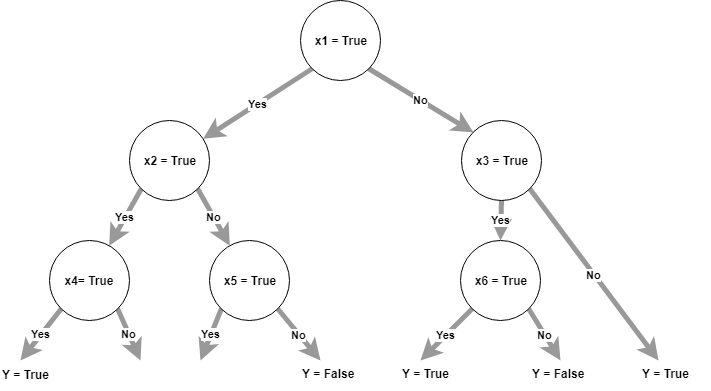
\includegraphics[width=0.75\textwidth]{design_and_methodology/decisiontree.png}}
\caption{\label{fig:mlp} Decision Tree Example}
\end{figure}

The DT Classifier was implemented with Scikit Learn with the following parameters:

\begin{tcolorbox}
\begin{center}
	DecisionTreeClassifier (criterion='entropy', max\_depth=32, max\_features=None, min\_samples\_leaf=2, min\_samples\_split=0.1)
\end{center}
\end{tcolorbox}

\subsubsection*{Random Forest}

%[B2001]	Breiman, “Random Forests”, Machine Learning, 45(1), 5-32, 2001.

The Random Forest Classifier (RF) is an ensemble classification algorithm, meaning it combines multiple base classification algorithms. It consists of multiple decision trees. The final class prediction is calculated by getting the average of the decision of the individual decision trees.

The RF Classifier was implemented with Scikit Learn with the following parameters:

\begin{tcolorbox}
\begin{center}
	RandomForestClassifier (n\_estimators=500, max\_features='log2',criterion='entropy')
\end{center}
\end{tcolorbox}

\subsubsection*{Multi Layer Perceptron}

\begin{figure}[h!]
\centering
\fbox{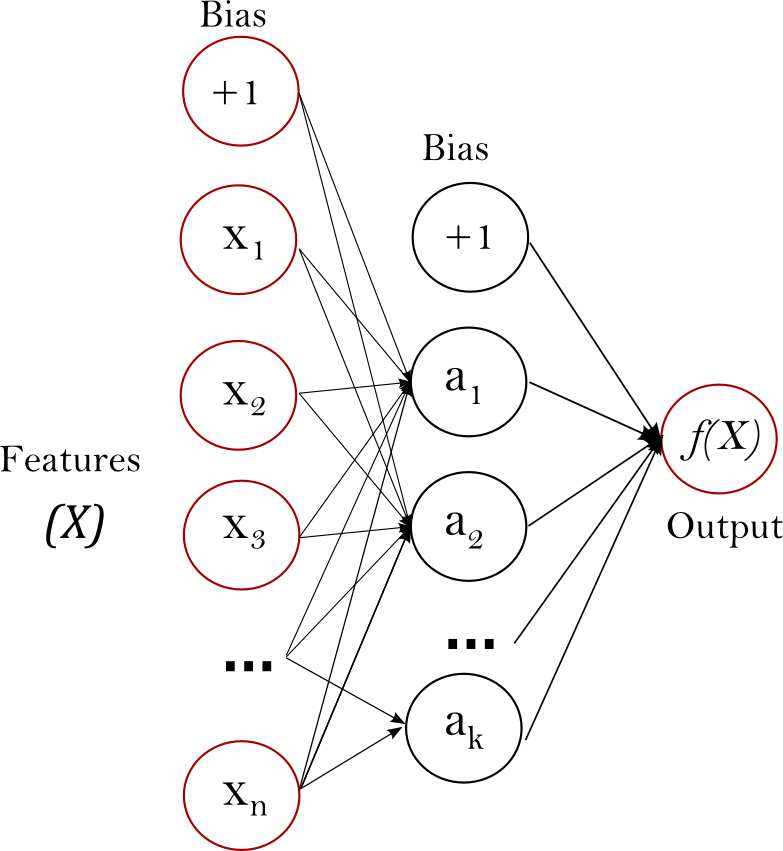
\includegraphics[width=0.5\textwidth]{design_and_methodology/multilayerperceptron_network.png}}
\caption{\label{fig:mlp} MLP with one hidden layer \cite{scikit-learn}}
\end{figure}

The Multi Layer Perceptron (MLP) Classifier is a deep, feedforward, artificial neural network. It conists of a minimum of three layers (Figure ~\ref{fig:mlp}); an input layer, a hidden layer and an output layer. The input layer receives the data, the output layer makes a decision and the hidden layers approximate the function.

The MLP learns a function by based on the training set. Given a set of features X = x1,x2,x3,...,xn and a target y, it learns a non-linear approximation function. Backpropagation is used to train the MLP.

The MLP Classifier was implemented with Scikit Learn with the following parameters:

\begin{tcolorbox}
\begin{center}
	MLPClassifier (alpha=1,activation='identity', hidden\_layer\_sizes=(100,), learning\_rate='constant', solver='adam')
\end{center}
\end{tcolorbox}

\subsubsection*{Support Vector Machine}

The Support Vector Machine (SVM) Classifier is a discriminative classifier. It finds the optimum hyperplane that separates the data into the labelled classes. It aims to maximise the distance between the hyperplane and the support vectors (the points closest to the hyper plane).

\begin{figure}[h!]
\centering
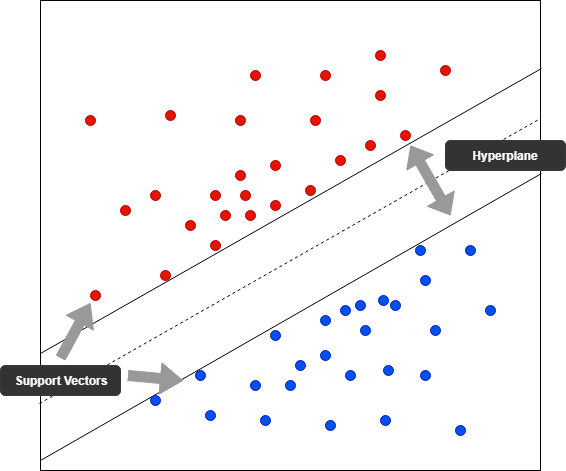
\includegraphics[width=0.75\textwidth]{design_and_methodology/svm.png}
\caption{\label{fig:svm} SVM.}
\end{figure}

The SVM Classifier was implemented with Scikit Learn with the following parameters:

\begin{tcolorbox}
\begin{center}
	SVC (C=10.1,decision\_function\_shape='ovo',degree=1,gamma=1,kernel='rbf')
\end{center}
\end{tcolorbox}

\subsubsection*{Logistic Regression}

The Linear Regression (LR) Classifier is a linear classification algorithm that uses the logistic function to model the training data. The logistic function is as follows:
\begin{center}
  \(g(z)=1/(1+e^{-z})\)  
\end{center}

The LR Classifier was implemented with Scikit Learn with the following parameters:

\begin{tcolorbox}
\begin{center}
	LogisticRegression (C=1,multi\_class='multinomial',penalty='l2',solver='saga')
\end{center}
\end{tcolorbox}

\subsubsection*{K Nearest Neighbours}

The K Nearest Neighbours (KNN) Classifier doesn't build a model like other classification algorithms. It uses a majority vote of the "nearest neighbours" to a document. A label is assigned to a document based on the class that has the majority of the nearest neighbours to the document. For example, point one would be assigned the label blue. Taking it's four nearest neighbours it has three blue neighbours and one red neighbour. The point is assigned to the class with the majority of the nearest neighbour, blue.

\begin{figure}[h!]
\centering
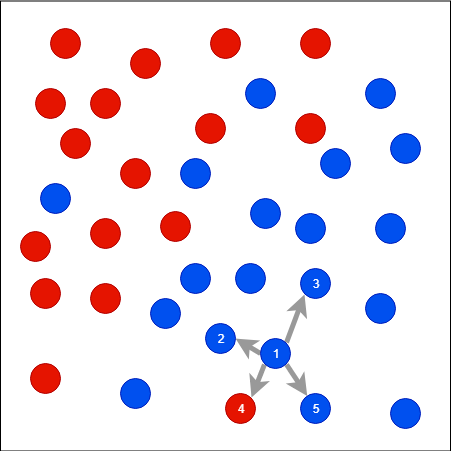
\includegraphics[width=0.7\textwidth]{design_and_methodology/knn.png}
\caption{\label{fig:knn} K Nearest Neighbours.}
\end{figure}

The KNN Classifier was implemented with Scikit Learn with the following parameters:

\begin{tcolorbox}
\begin{center}
	KNeighborsClassifier(n\_neighbors=17,algorithm='ball\_tree',weights='distance',
	leaf\_size=10,p=2)
\end{center}
\end{tcolorbox}

\subsubsection*{Gaussian Process}

The GP Classifier was implemented with Scikit Learn with the following parameters:

\begin{tcolorbox}
\begin{center}
	GaussianProcessClassifier(1.0 * RBF(1.0))
\end{center}
\end{tcolorbox}

\subsubsection*{Adaboost}

The AdaBoost Classifier was implemented with Scikit Learn with the following parameters:

\begin{tcolorbox}
\begin{center}
	AdaBoostClassifier()
\end{center}
\end{tcolorbox}

\subsubsection*{Gaussian Naive Bayes}

The Gaussian NB Classifier was implemented with Scikit Learn with the following parameters:

\begin{tcolorbox}
\begin{center}
	GaussianNB()
\end{center}
\end{tcolorbox}

\subsubsection*{Bernoulli Naive Bayes}

The Bernoulli NB Classifier was implemented with Scikit Learn with the following parameters:

\begin{tcolorbox}
\begin{center}
	BernoulliNB()
\end{center}
\end{tcolorbox}

\subsubsection*{Quadratic Discriminant Analysis}

The QDA Classifier was implemented with Scikit Learn with the following parameters:

\begin{tcolorbox}
\begin{center}
	QuadraticDiscriminantAnalysis()
\end{center}
\end{tcolorbox}

\subsubsection*{Linear Discriminant Analysis}

The LDA Classifier was implemented with Scikit Learn with the following parameters:

\begin{tcolorbox}
\begin{center}
	LinearDiscriminantAnalysis()
\end{center}
\end{tcolorbox}


\section{Sentiment Analysis}

\subsection*{The Stanford Sentiment Analyser}
%Limitations - data it was trained on etc.
\subsection*{Normalising the Sentiment Scores}

\section{CoRE Recommender System}

The sentiment scores produced by the Stanford Sentiment Analyser were used to re rank the list of hotel recommendations produced by the CoRE recommender system.

